\documentclass{book}

\usepackage{tikz}
\usepackage{tkz-euclide}
\usepackage{nicematrix}
\usepackage{geometry,setspace}
\usepackage[utf8x]{inputenc}
\usepackage[russian,english]{babel}
\usepackage{graphicx}
\usepackage{hyperref}
\usepackage{import}
\usepackage{amsmath, amssymb}
\usepackage{fancybox, fancyhdr}
\usepackage{graphicx}
\usepackage{blindtext}
\usepackage{ragged2e}

\renewcommand*{\thesection}{\arabic{section}}
\newtheorem{theorem}{Теорема}
\newtheorem{definition}{Определение}
\newtheorem{follows}{Следствие}
\newtheorem{lemm}{Лемма}
\newtheorem{note}{Замечание}

\begin{document}
	\selectlanguage{Russian}
	
	
	\begin{titlepage}
		\centering
		
		\vspace*{2cm}
		
		{\Huge\bfseries Коллоквиум по}
		{\Huge\bfseries математическому анализу III}
		
		{\Huge\bfseries Второй поток}
		
		\vspace*{2.2cm}
		
		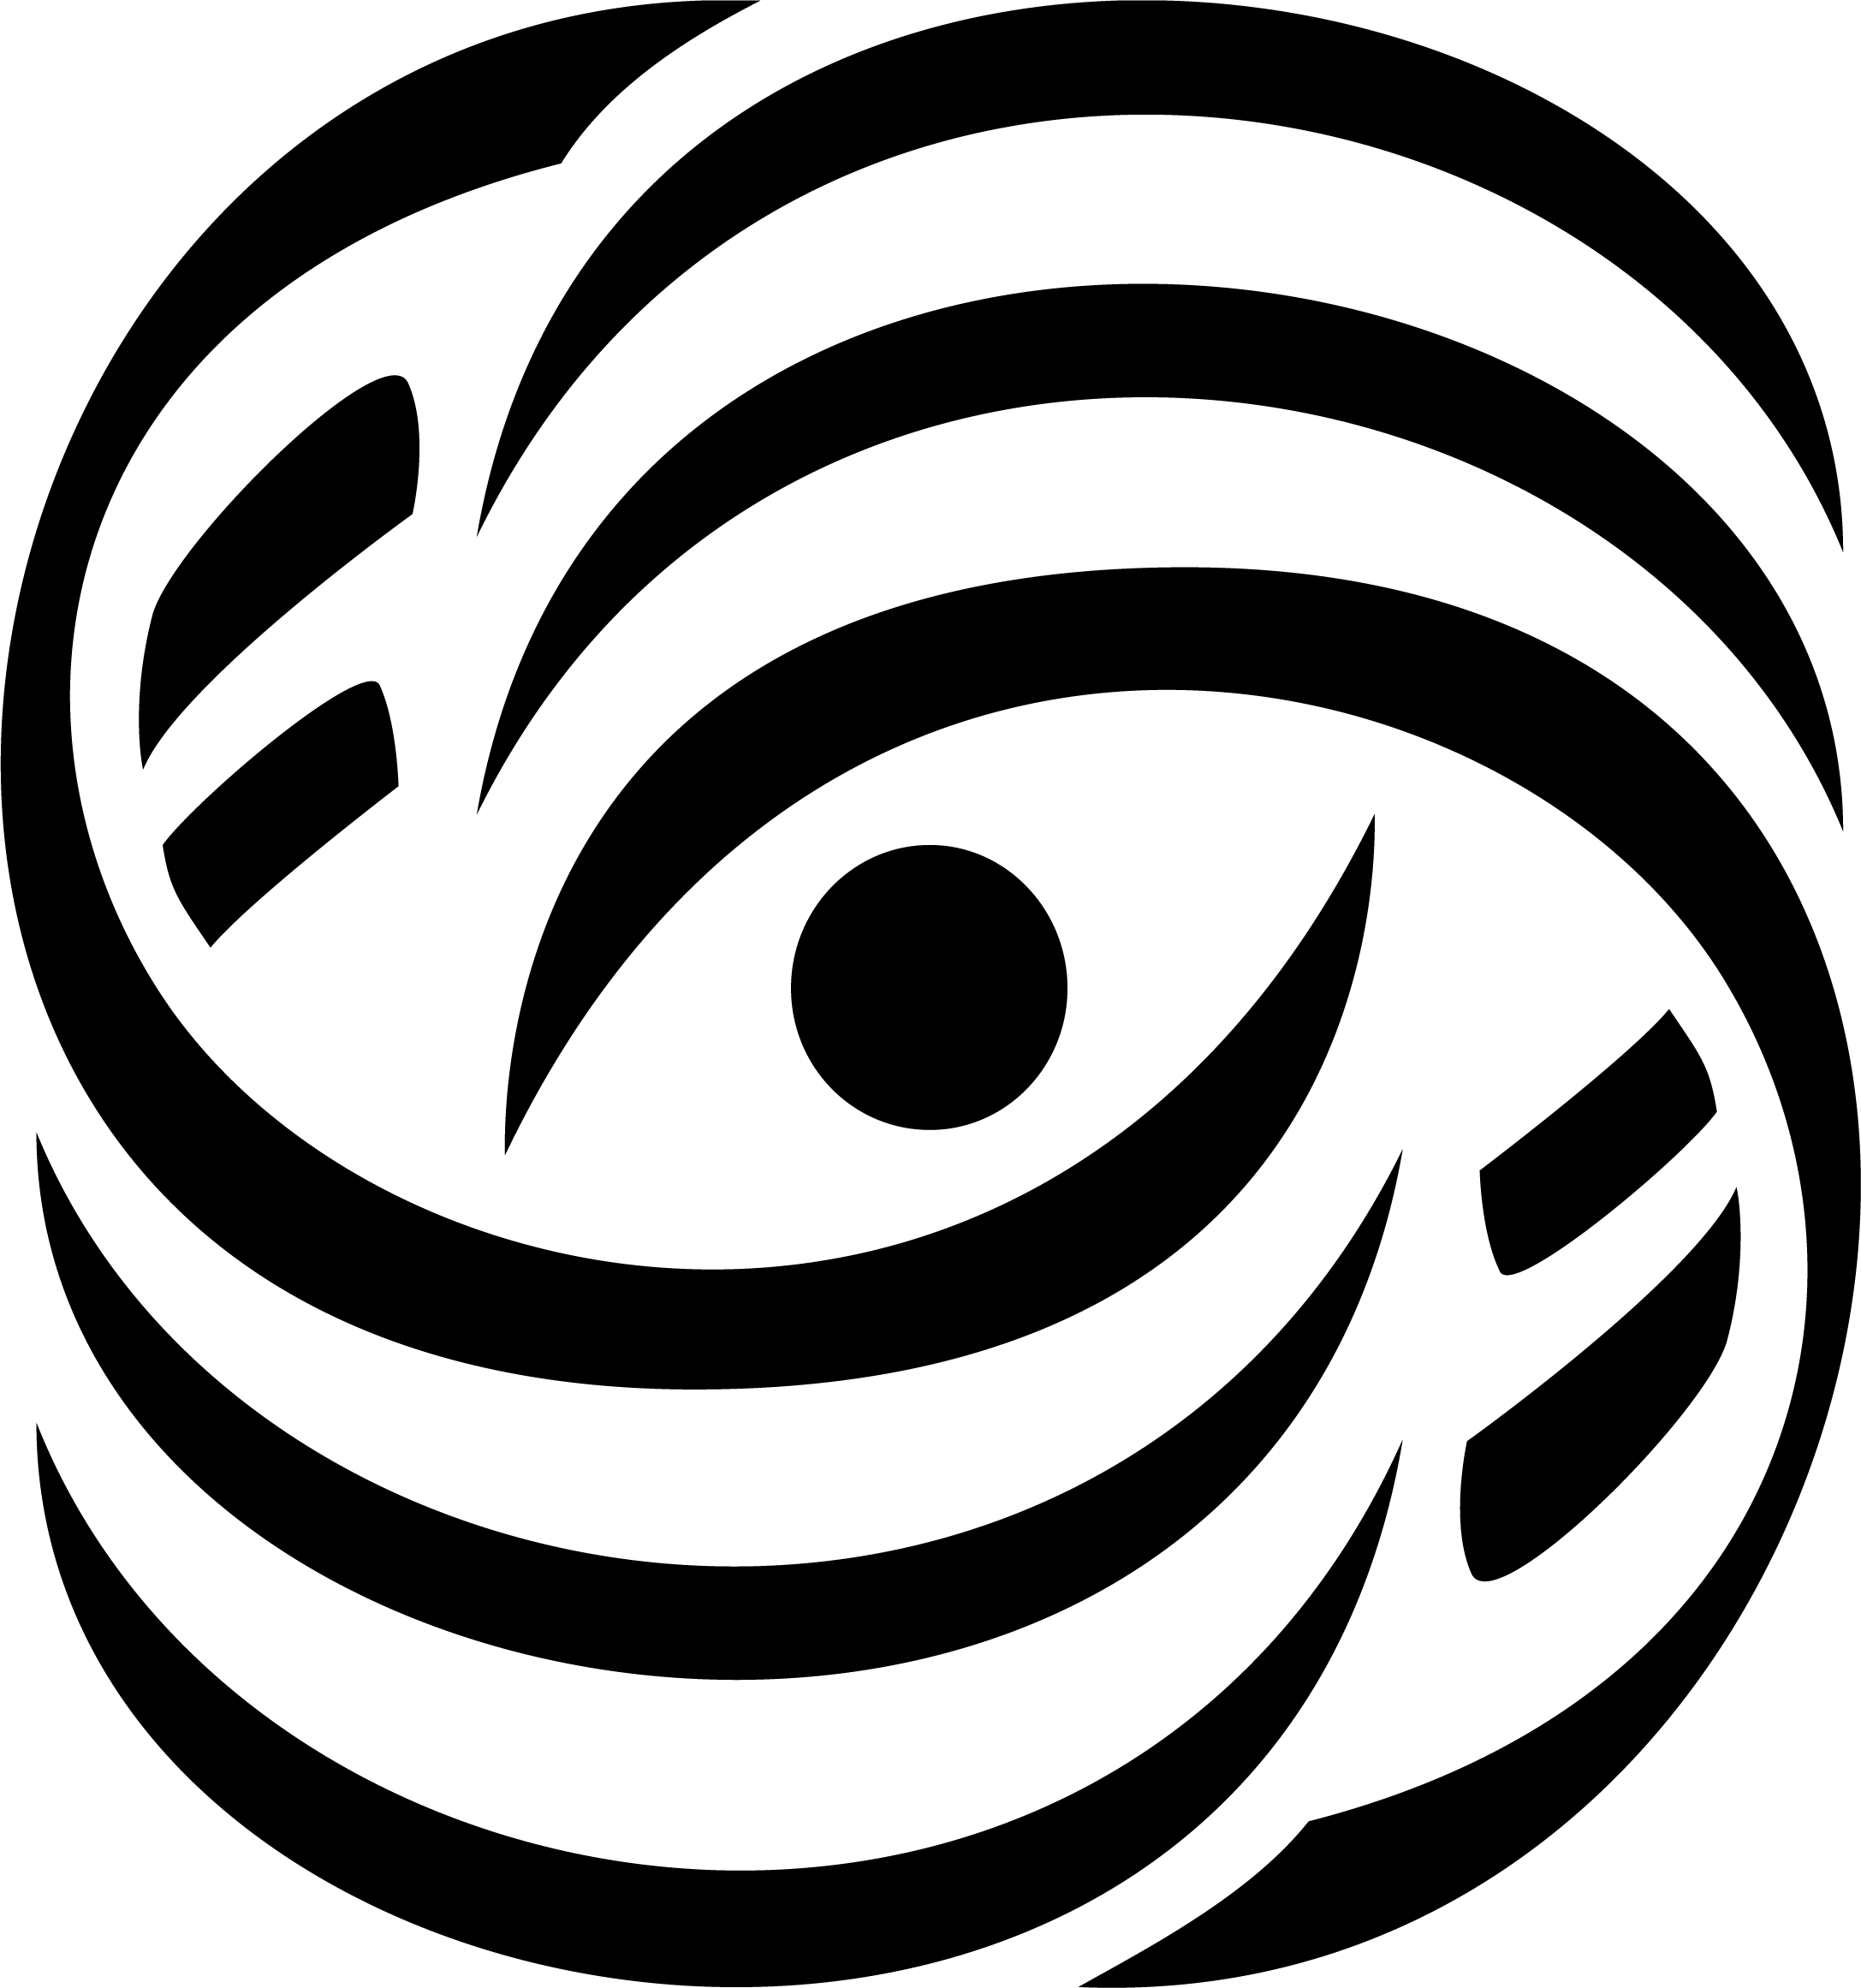
\includegraphics[width=0.6\textwidth]{logo.png}
	\end{titlepage}
	
	\thispagestyle{empty}
	\tableofcontents
	\thispagestyle{empty}
	\clearpage
	
	\pagestyle{fancy}
	\setcounter{page}{1}
	\fancyhf{}
	\fancyhead[LE]{\thepage}
	\fancyhead[RO]{\thepage}
	
	\import{./}{q1.tex}
	\section*{Признаки сходимости рядов с неотрицательными членами}
	\import{./}{q2.tex}
	\import{./}{q3.tex}
	\import{./}{q4.tex}	
	
\end{document}